% ECSE 552 final report (20%), due December 6, 2026 at 23:59.
% Length: ~5,000--8,000 words excluding references. The main report must be
% self-contained; supplementary material only for details a grader may need.
% C1--C11 below are the instructor's required elements; see docs/course-requirements.md.
% Every number comes from docs/experiments/*.md or the dataset manifests; pending items
% are marked with \todo and must stay visible until they are filled.
\documentclass{article}

\PassOptionsToPackage{numbers,sort&compress}{natbib}
\usepackage[preprint]{neurips_2026}
% Course document, not a preprint: drop the "Preprint." notice on page 1.
\makeatletter\renewcommand{\@noticestring}{}\makeatother
\usepackage[utf8]{inputenc}
\usepackage[T1]{fontenc}
\usepackage{hyperref}
\usepackage{url}
\usepackage{booktabs}
\usepackage{array}
\usepackage{amsfonts}
\usepackage{amsmath}
\usepackage{microtype}
\usepackage{graphicx}
\usepackage{xcolor}

\newcommand{\todo}[1]{\textcolor{red}{[TODO: #1]}}

\title{Learning to Manipulate a New Object\\from Action-Free Videos}

\author{
  Group 9: Brik Meza, Myriam Dardour, Zheng Ye Zhang, Gonzalo Mill\'an Garc\'ia \\
  McGill University \\
  ECSE 552 --- Final report (draft)
}

\begin{document}

\maketitle

\begin{abstract}
  Visuomotor policies imitate images paired with motor commands, and every new object
  normally requires new paired demonstrations. We study whether videos without actions are
  enough to extend an image-only policy from one object to another. In simulation
  (OCBench, UR5e arm), labeled demonstrations exist only for a red source cube; each
  target object has only videos. An inverse dynamics model (IDM), trained on the source
  and adapted to the target with domain-adversarial training (DANN), labels the target
  videos, and an image-only ACT policy trains on both. In preliminary single-seed
  results, the source-only policy solves the source cube from images alone (99\% test
  success, 10~ms per inference call) but fails when only the cube's colour changes (7\%),
  which leaves a large gap for the action-free methods to close.
  \todo{Results of the IDM methods against the baselines, R4 and R5, and the conclusion.}
\end{abstract}

\section{Introduction}
% C1: define the application.
% C2: high-level problem formulation.
% C3: why a solution is needed; contextualize and cite related work.
% C4: constraints important to the application and problem.

\paragraph{Application (C1).}
Warehouse and home robots meet new items constantly. A robot arm that already manipulates
one object should learn to handle a new one without anyone operating the robot again.
We study this for a tabletop pick-and-place task in the OCBench simulator
\citep{ocbench2026}, built on MuJoCo \citep{todorov2012mujoco}: a UR5e arm with a Robotiq
gripper picks up a block and places it inside a goal square, seeing the scene only
through three RGB cameras (Figure~\ref{fig:scene}).

\begin{figure}[t]
  \centering
  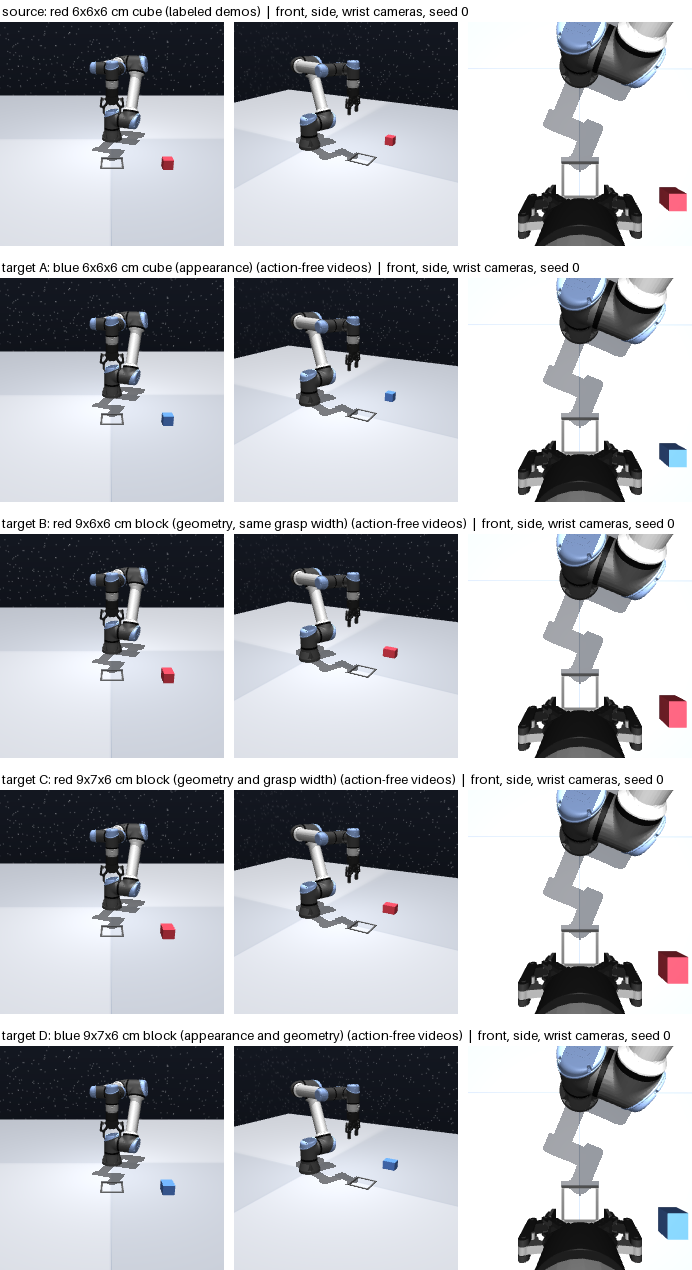
\includegraphics[width=\linewidth]{../scene.png}
  \caption{Initial state seen by the front, side and wrist cameras, for the red source
  cube and the blue target A. The gray square is the goal.}
  \label{fig:scene}
\end{figure}

\paragraph{Why a solution is needed (C3).}
Visuomotor policies such as ACT \citep{zhao2023act} and Diffusion Policy
\citep{chi2023diffusionpolicy} imitate images paired with motor commands. Acquiring such
pairs is costly because it requires operating the robot: 50 people took a year to collect
the 76k teleoperated demonstrations of DROID \citep{khazatsky2024droid}. With limited
coverage, a policy that meets an unfamiliar situation may output an erroneous action, and
errors compound during execution, moving the robot further from its training data
\citep{zhao2023act}. Videos are far cheaper than paired data: they can be recorded
without logging commands, and world models can now generate them
\citep{jang2025dreamgen}. The open question is how to turn videos into supervision for a
policy that must output motor commands.

\paragraph{Related work.}
The standard recipe trains an \emph{inverse dynamics model} (IDM) on transitions with
known actions, uses it to label observation-only demonstrations, and clones the result:
behavioral cloning from observation \citep{torabi2018bco}, scaled to internet video by
VPT \citep{baker2022vpt} and to video generated by world models by DreamGen
\citep{jang2025dreamgen}. \citet{morin2026idmssil} analyse why this is sample efficient
with few labels and name unlabeled data from a different environment as future work;
this is our setting. \citet{kim2023givinghand} label human eye-in-hand videos with an
IDM trained on robot play. A second line avoids explicit pseudo-actions by learning
latent actions or motion representations from videos
\citep{ye2025lapa,collins2025amplify,nikulin2025laom}; these methods need larger models
and data than this project allows. When the videos show a new object, the IDM is applied
outside its training distribution. Unsupervised domain adaptation addresses this
shift by aligning source and target features, adversarially in DANN
\citep{ganin2016dann} and its successors \citep{tzeng2017adda,long2018cdan}. Alignment
has been applied to the policy's encoder for visuomotor transfer
\citep{cheng2025gda,kato2026udail}, but \citet{cheng2025gda} require action-labeled
target demonstrations. Two warnings apply to our design: invariant features can hurt
when the label distribution differs between domains \citep{zhao2019invariant}, and
adversarial alignment was designed for classification and is weaker for regression
\citep{nejjar2023daregram}. We found no work that adapts an IDM adversarially to
pseudo-label action-free videos of a new object for the same robot; we frame this as a
controlled study and not as a new method.

\paragraph{Problem (C2, high level).}
Labeled demonstrations (images and actions) exist only for a \emph{source} object.
For each \emph{target} object there are only videos. We want one image-only policy per
target that succeeds on the target without losing the source, and we ask whether
adapting the IDM to the target before labeling its videos helps.

\paragraph{Scope.}
The source is a $6 \times 6 \times 6$~cm red cube. Targets are (A) a blue cube of the
same size (appearance), (B) a $9 \times 6 \times 6$~cm red block (geometry, same grasp
width), (C) a $9 \times 7 \times 6$~cm red block (geometry and grasp width) and,
optionally, (D) a blue version of C. Robot, cameras, lighting and task stay fixed. Human
videos, large pretrained models and real robots are out of scope.
\todo{State which targets were completed; this draft has results for the source and A only.}

\subsection{Constraints}
% C4.
Table~\ref{tab:requirements} lists the requirements the design must satisfy (C4). R1--R3
define the supervision contract and hold by construction; R4 and R5 are the outcome
targets; R6 is the real-time condition. R6 was restated when the control rate changed
(Section~\ref{sec:solution}): the policy is queried at every 10~Hz control step, so one
call must finish within the 100~ms control period.

\begin{table}[t]
  \caption{Requirements (C4) and their status in this draft. Baseline numbers are from a
  single training seed and are preliminary.}
  \label{tab:requirements}
  \centering
  \small
  \begin{tabular}{@{}>{\raggedright\arraybackslash}p{0.5cm}>{\raggedright\arraybackslash}p{1.7cm}>{\raggedright\arraybackslash}p{4.4cm}>{\raggedright\arraybackslash}p{2.1cm}>{\raggedright\arraybackslash}p{3.5cm}@{}}
    \toprule
    ID & Requirement & Definition & Target & Status \\
    \midrule
    R1 & Supervision & Target data are RGB frames only & Zero target labels &
      By design; \todo{confirm for the IDM pipeline} \\
    R2 & Label budget & Labeled source demonstrations, identical for every method &
      100; 300 if the source-only policy is below 80\% in source validation &
      Pending: 300 demos reach 98\% in validation; \todo{100-demo result and decision} \\
    R3 & Inputs & No simulator state in any learned model & Images only &
      Met by the policy (robot state zeroed); \todo{IDM} \\
    R4 & Target & Success gain over the source-only policy on each target, as a fraction
      of the oracle's gain & $\geq 50\%$ of the gap & \todo{R4 per target} \\
    R5 & Retention & Drop in source success after adding target data & $\leq 10$ points &
      \todo{R5 per target} \\
    R6 & Real time & Policy inference per call, within one 10~Hz control step (IDM
      offline) & $< 100$~ms & Measured: 10~ms (95th percentile) \\
    \bottomrule
  \end{tabular}
\end{table}

\section{Methods}

\subsection{Problem formulation}
% C2 in detail.
An episode is a sequence of observations $o_t$ (three RGB images) and actions
$a_t \in \mathbb{R}^7$ (six arm joints and the gripper). The source dataset contains
labeled transitions, $\mathcal{D}_S = \{(o_t, a_t, o_{t+1})\}$, from $N_S$ demonstrations
of the source object. Each target $T \in \{\mathrm{A, B, C, D}\}$ has only videos,
$\mathcal{D}_T = \{o_t\}$. Source and target share the robot, the cameras, the task and
the expert's strategy; they differ in the object's appearance or geometry, so the
observation distribution shifts and, for geometry changes, the action distribution may
shift as well.

We seek, for each target, an image-only policy $\pi_T(a_{t:t+H} \mid o_t)$ that predicts a
chunk of $H$ future actions. Let $s(\pi, X)$ be the closed-loop success rate of policy
$\pi$ on object $X$. Three reference policies anchor the requirements: $\pi_a$ trained
on $\mathcal{D}_S$ only, $\pi_d$ trained on $\mathcal{D}_S$ plus the target with its
true actions (oracle), and the candidate $\pi_T$ trained on $\mathcal{D}_S$ plus
pseudo-labeled $\mathcal{D}_T$. R4 and R5 are
\begin{align}
  \text{R4:}\quad & G_T = \frac{s(\pi_T, T) - s(\pi_a, T)}{s(\pi_d, T) - s(\pi_a, T)} \geq 0.5,
  \label{eq:r4} \\
  \text{R5:}\quad & s(\pi_a, S) - s(\pi_T, S) \leq 0.10 .
  \label{eq:r5}
\end{align}
R4 is inconclusive for a target if the oracle does not exceed the source-only policy,
$s(\pi_d, T) \leq s(\pi_a, T)$. True target actions are used only to train the oracle
and to evaluate pseudo-label error; they never select a model (R1).

\subsection{Datasets and resources}
\label{sec:data}
% C5.
All data are generated by us in simulation; no licensing or ethics constraints apply.

\paragraph{Scene and task.}
We use OCBench's visual single-block task (\texttt{visual-block-cpu-lite-single-task1-v0})
through our fork of the simulator, which adds cube colours, a visible goal and
reproducible initial states. A dark-gray 12~cm square marks the fixed goal. An episode
succeeds when the whole object is inside the square, resting on the table, released and
still for 1~s; the time limit is 200 control steps (20~s). The object starts uniformly in
a $20 \times 20$~cm area beside the goal with its yaw fixed at 0, and the arm always
starts from the same pose. The 12~cm side was chosen from the expert's own precision: 97\%
of its resting placements fit fully inside a 12~cm square, against 60\% for 8~cm (200
episodes).

\paragraph{Observations and actions.}
Each control step (10~Hz) stores one $224 \times 224$ RGB image from each of the front,
side and wrist cameras. OCBench actions are seven values in $[-1, 1]$: six arm-joint
increments and one gripper-opening increment, each added to the current measured
position. Simulator state (joint positions and velocities) is stored for replay,
evaluation and label conversion, but is never an input of a learned model (R3).

\paragraph{Collections and seeds.}
Demonstrations come from OCBench's scripted expert. Every episode has its own seed,
which fixes the initial state and the expert's random choices; failed attempts are
discarded and recorded. Seed ranges do not overlap (Table~\ref{tab:collections}), and the
same seed gives the same initial object and arm state for every object, so all methods
are evaluated from identical initial states. We verified that stored episodes replay exactly from
their actions.

\begin{table}[t]
  \caption{Collections and seed ranges, fixed before any result. Demonstrations average
  76 steps (7.6~s).}
  \label{tab:collections}
  \centering
  \small
  \begin{tabular}{@{}llrl@{}}
    \toprule
    Collection & Seeds from & Episodes & Use \\
    \midrule
    Source demonstrations & 0 & 300 & Training and validation, labeled \\
    Source, held out & 50,000 & 50 & IDM test error only \\
    Target A videos & 100,000 & 200 & Action-free; true actions: oracle, evaluation \\
    Target B, C, D videos & 200,000+ & \todo{200 each} & Same as A \\
    Validation rollouts & 900,000 & 100 & Checkpoint selection, R2 (source only) \\
    Test rollouts & 1,000,000 & 100 & Final evaluation, every object \\
    \bottomrule
  \end{tabular}
\end{table}

\paragraph{Deterministic against stochastic demonstrations.}
Stock OCBench demonstrations are deliberately varied: the cube has a random yaw, and the
expert moves at a random speed and takes deliberate detours. We collected both this
\emph{stochastic} variant and a \emph{deterministic} one (yaw fixed at 0, no detours,
fixed speed), with the same seeds. The same unmodified ACT, trained on 300 source
demonstrations with one seed, reaches 99\% test success on the deterministic data and
53\% on the stochastic data (Section~\ref{sec:results}). Evaluating the stochastic policy
from fixed-yaw starts gives 71\% in validation, so about 18 points of the gap come from
the harder initial states and about 27 from the variability of the demonstrations. We
therefore fixed the deterministic data as the project data for every method and object,
before running any method that uses target videos: the research question concerns the
transfer between objects, and a source-only policy that fails half the time on its own
object would leave no room to measure retention (R5) or a meaningful oracle gap (R4).
The stochastic collections are kept as a reference. The deterministic expert is not
fully deterministic: it keeps OCBench's grasp randomness (a $\pm 90^\circ$ wrist mode in
30\% of episodes, a pick hold in 40\% and about 1~cm of contact jitter). Its success rate
is 99.7\% on the source (300 of 301 attempts) and 100\% on target A.

\paragraph{Resources.}
Episodes are public on the Hugging Face Hub
(\url{https://huggingface.co/datasets/Autobrik/ecse552-ocbench-block}); training
downloads a pinned revision, and checkpoints are published in companion model
repositories. A LeRobot copy \citep{cadene2024lerobot} serves the online visualizer.
Policies train on Modal with one NVIDIA A10G GPU, about 2~h per ACT run, with curves
logged to Weights~\&~Biases. Rendering and rollouts run on a local GPU. The code is at
\url{https://github.com/BrikHMP18/ecse-552-project}.

\subsection{Designed solution and implementation}
\label{sec:solution}
% C6.
The pipeline has three stages: (1) train an IDM on labeled source transitions, adapting
it to the target with DANN; (2) label the target videos with the IDM; (3) train an
image-only ACT policy on source demonstrations plus pseudo-labeled target videos. One
policy is trained per target. IDM and policy share no weights.

\paragraph{Inverse dynamics model.}
The IDM $f_\theta$ predicts the action between two consecutive observations,
$\hat{a}_t = f_\theta(o_t, o_{t+1})$. A convolutional encoder shared across cameras embeds
both frames and their difference, which exposes motion and suppresses static appearance;
an MLP regresses the action with a mean-squared-error loss on source transitions,
\begin{equation}
  \mathcal{L}_{\text{act}}(\theta) = \mathbb{E}_{(o_t, a_t, o_{t+1}) \sim \mathcal{D}_S}
  \big\| f_\theta(o_t, o_{t+1}) - a_t \big\|_2^2 .
\end{equation}
The IDM is easier to learn from few labels than the policy because it does not need to
model the expert's intent, only the effect of an action that already happened
\citep{morin2026idmssil}. Its split takes blocks of ten source episodes, eight for
training and two for validation.
\todo{IDM architecture (encoder, input resolution, output: absolute joint targets),
optimizer, training length and source validation error.}

\paragraph{Domain-adversarial adaptation.}
Following DANN \citep{ganin2016dann}, a domain discriminator $d_\phi$ receives the IDM's
features $h_\theta$ for source and target frame pairs and is trained with binary
cross-entropy to tell them apart. A gradient reversal layer makes the encoder maximize
the same loss, scaled by $\lambda$:
\begin{equation}
  \min_{\theta} \max_{\phi} \;\; \mathcal{L}_{\text{act}}(\theta) -
  \lambda \, \mathcal{L}_{\text{dom}}(\theta, \phi), \qquad
  \mathcal{L}_{\text{dom}} = \mathrm{BCE}\big(d_\phi(h_\theta(o_t, o_{t+1})),\, y_{\text{dom}}\big).
\end{equation}
The encoder is thus pushed towards features that predict source actions but do not
reveal the domain. $\lambda$ ramps up on a schedule fixed in advance, and $\lambda = 0$
gives the unadapted IDM of method (b). Only target \emph{frames} enter this stage (R1).
IDM checkpoints are selected by source validation error, never with target actions.
\todo{Discriminator architecture, $\lambda$ schedule and final value, batch composition.}

\paragraph{Policy.}
The policy is the original ACT \citep{zhao2023act}, run from the authors' code without
modification through a thin adapter. ACT is a conditional VAE: a ResNet-18 backbone per
camera feeds a transformer encoder (4 layers) and decoder (7 layers, 8 heads, hidden
size 512, feed-forward size 3,200) that outputs a chunk of $H = 20$ actions (2~s); a
separate encoder maps the action chunk to a 32-dimensional latent $z$ during training,
and $z = 0$ at test time. The loss is
\begin{equation}
  \mathcal{L}_{\text{ACT}} = \big\| \hat{a}_{t:t+H} - a_{t:t+H} \big\|_1 +
  \beta \, D_{\mathrm{KL}}\big( q(z \mid a_{t:t+H}, o_t) \,\|\, \mathcal{N}(0, I) \big),
  \qquad \beta = 10 .
\end{equation}
We keep the hyperparameters of the ACT repository (batch size 8, learning rate
$10^{-5}$, weight decay $10^{-4}$, 2,000 epochs). The only change is that the robot-state
input is set to zero, so the policy sees images only (R3).

\paragraph{Actions and execution.}
Policies are trained on absolute joint targets, computed from the stored increments and
joint positions: $q^{\ast}_t = q_t + a_t \odot c$ for the arm, with $c$ the simulator's
per-joint scale, and the clipped opening for the gripper. A low-level controller converts
each target back into the increment the simulator expects. At test time the policy is
queried at every step and the overlapping chunks are combined by ACT's temporal
ensembling: the executed target is $\sum_i w_i \hat{q}^{(i)}_t / \sum_i w_i$ with
$w_i = \exp(-k\,i)$, $k = 0.01$, where $i = 0$ is the oldest prediction for step $t$.

\paragraph{Deviations from the proposal.}
Table~\ref{tab:deviations} lists the decisions that differ from the proposal. Most
follow from one finding: our first policy, a reimplementation of ACT with the proposal's
settings (joint increments, open-loop chunks, stochastic data), did not exceed 49\%
validation success on the source cube (Section~\ref{sec:whatwentwrong}). We replaced it
with the original ACT and adopted its conventions.

\begin{table}[t]
  \caption{Decisions that differ from the proposal.}
  \label{tab:deviations}
  \centering
  \small
  \begin{tabular}{@{}>{\raggedright\arraybackslash}p{1.6cm}>{\raggedright\arraybackslash}p{3.0cm}>{\raggedright\arraybackslash}p{2.6cm}>{\raggedright\arraybackslash}p{5.4cm}@{}}
    \toprule
    Topic & Decision & Proposal & Reason \\
    \midrule
    Control rate & 10~Hz, at most 200 steps; chunk 20 (2~s) & 50~Hz, chunk 25 &
      One image per control step; the chunk keeps ACT's 2~s horizon \\
    Actions & Absolute joint targets & Joint increments &
      ACT's convention; increments assume the state they were predicted from, so
      re-querying or averaging them fails \\
    Execution & Temporal ensembling & Chunks open loop &
      Open loop gives 41\% against 98\% for the same policy
      (Table~\ref{tab:execution}) \\
    Initial state & Object yaw fixed at 0; $20 \times 20$~cm start area; fixed arm pose &
      OCBench defaults & As in ACT's simulated tasks; isolates the object shift \\
    Expert & Deterministic: no detours, fixed speed & OCBench's, adapted per object &
      99\% against 53\% source success (Section~\ref{sec:data}) \\
    Goal & 12~cm square; inside, resting, released, still for 1~s & Within 4~cm &
      A visible goal and a strict success test \\
    Policy & Original ACT code; checkpoint chosen by validation rollouts &
      Own ACT, fixed training steps &
      Our reimplementation underperformed; validation loss picks poor checkpoints \\
    Split & 80/20 train/validation by episode; test by rollouts on reserved seeds &
      80/10/10 & Upstream ACT's split; success needs rollouts, not held-out demos \\
    R6 & $< 100$~ms per call & $< 0.5$~s per chunk &
      Temporal ensembling queries the policy every step \\
    \bottomrule
  \end{tabular}
\end{table}

\subsection{Evaluation}
\label{sec:evaluation}
% C7: splits, metrics, and evaluation protocol.
The protocol was fixed in the repository's configuration before any result.

\paragraph{Splits.}
Source demonstrations are split by episode into 80\% training and 20\% validation (ACT's
own random split). Fifty held-out source demonstrations (seeds 50,000+) are used only for
the IDM's test error. Closed-loop evaluation uses two disjoint seed ranges shared by
all methods and objects: validation rollouts (seeds 900,000+) and test rollouts (seeds
1,000,000+).

\paragraph{Checkpoint selection.}
Each ACT run saves the checkpoint with the lowest validation loss (\emph{best}) and the
final one (\emph{last}). We run 100 validation rollouts on the \emph{source} object for
each and keep the one with higher success, with ties going to \emph{best}. Selection
never uses the target's actions or the target's success, so R1 holds for model selection
too. The R2 decision (100 or 300 demonstrations) uses the same validation rollouts.

\paragraph{Test.}
Each selected checkpoint is evaluated once: 100 test rollouts per object, from the same
initial states for every method. Each method is trained with three seeds; we report
the mean and standard deviation across seeds and, for each success rate, the 95\% Wilson
score interval. For $k$ successes in $n$ rollouts, $\hat{p} = k/n$ and $z = 1.96$,
\begin{equation}
  \frac{\hat{p} + \frac{z^2}{2n} \pm z \sqrt{\frac{\hat{p}(1 - \hat{p})}{n} + \frac{z^2}{4n^2}}}{1 + \frac{z^2}{n}} .
\end{equation}
Intervals are necessary beyond sampling error: GPU rendering is not bit-exact, so
rerunning the same seeds changes some outcomes (Section~\ref{sec:discussion}).

\paragraph{Metrics.}
(i) Success rate on each target and on the source, from which R4 (Eq.~\ref{eq:r4}) and R5
(Eq.~\ref{eq:r5}) follow. (ii) Inference latency per policy call during rollouts, after
warm-up, reported as the 95th percentile (R6). (iii) IDM error per action component on
held-out source transitions and, with the true target actions, pseudo-label error on the
target videos; the second is a diagnostic only. (iv) A classification of failed rollouts:
never lifted, placed just outside the goal, lifted and ended far, inside but not
released.

\subsection{Alternative solutions}
\label{sec:alternatives}
% C8: baselines, all run on our own data.
All alternatives are run on our own data with the same ACT architecture, training budget
and evaluation (Table~\ref{tab:methods}). Methods (a) and (d) anchor R4: the source-only
floor and the oracle with true target actions. Comparing (b) and (c) isolates the
effect of adapting the IDM, since they differ only in $\lambda$. Method (e) tests whether
target videos are needed at all: it trains on source data with hue, brightness, contrast
and saturation jitter and small random crops \citep{laskin2020rad}. We expect (e) to be
competitive on target A, where only colour changes, and weaker on B and C, whose
geometry and grasp width these augmentations do not reproduce. Optional method (f) moves
the alignment from the IDM to the policy's encoder \citep{kato2026udail}.

\begin{table}[t]
  \caption{Methods compared. All use the same source demonstrations and ACT policy.}
  \label{tab:methods}
  \centering
  \small
  \begin{tabular}{@{}llll@{}}
    \toprule
    & Method & Target data & Target labels \\
    \midrule
    (a) & Source only & None & None \\
    (b) & Unadapted IDM ($\lambda = 0$) & Videos & IDM pseudo-labels \\
    (c) & DANN-adapted IDM (ours) & Videos & IDM pseudo-labels \\
    (d) & Oracle & Demonstrations & True actions \\
    (e) & Source only with augmentation & None & None \\
    (f) & (b) with policy-encoder alignment (optional) & Videos & IDM pseudo-labels \\
    \bottomrule
  \end{tabular}
\end{table}

\section{Results}
\label{sec:results}
% C9: quantitative results and how the design meets the C4 constraints.
% C10: quantitative comparison against alternatives on C4.
\textbf{All numbers in this section come from one training seed and are preliminary.}
\todo{Replace with three seeds (mean, standard deviation) once the runs finish.}

\subsection{Source-only baseline (a)}
Table~\ref{tab:baseline} reports the original ACT trained on 300 source demonstrations.
On the project data the image-only policy reaches 99\% on the source cube, which meets
R3 and the 80\% level of R2 at 300 demonstrations. Changing only the cube's colour
breaks it: 7\% on target A. The floor of R4 is therefore near zero, and the methods that
use A's videos have a large gap to close. Inference takes 10~ms per call (95th
percentile), a tenth of the R6 budget.

\begin{table}[t]
  \caption{Baseline (a): original ACT, 300 source demonstrations, one seed. Validation
  and test success over 100 rollouts each; 95\% Wilson intervals in brackets. The
  robot-state run breaks R3 and is a reference only.}
  \label{tab:baseline}
  \centering
  \small
  \begin{tabular}{@{}llcccc@{\hspace{6pt}}c@{}}
    \toprule
    & & \multicolumn{2}{c}{Validation (source)} & \multicolumn{2}{c}{Test} & Latency \\
    \cmidrule(lr){3-4} \cmidrule(lr){5-6}
    Data & Input & best & last & Source & Target A & p95 \\
    \midrule
    Stochastic & Images & 40\% & 53\% & 53\% [43, 62] & 0\% [0, 4] & 10 ms \\
    Deterministic (project) & Images & 61\% & 98\% & \textbf{99\%} [95, 100] & \textbf{7\%} [3, 14] & 10 ms \\
    Deterministic & Images + state & 44\% & 66\% & 69\% [59, 77] & 1\% [0, 5] & 10 ms \\
    \bottomrule
  \end{tabular}
\end{table}

In all three runs the final checkpoint was selected: the checkpoint with the lowest
validation loss was always worse in rollouts (Figure~\ref{fig:curves}). On the source
cube, the selected deterministic policy fails once in 100 validation rollouts (cube
never lifted); the stochastic policy fails mostly by never lifting the cube (38) or
placing it just outside the goal (11). Adding the robot state did not help (69\%); its
success varies widely between nearby checkpoints, so one seed does not support a claim.
\todo{R2: validation success with 100 demonstrations and the resulting budget.}

\begin{figure}[t]
  \centering
  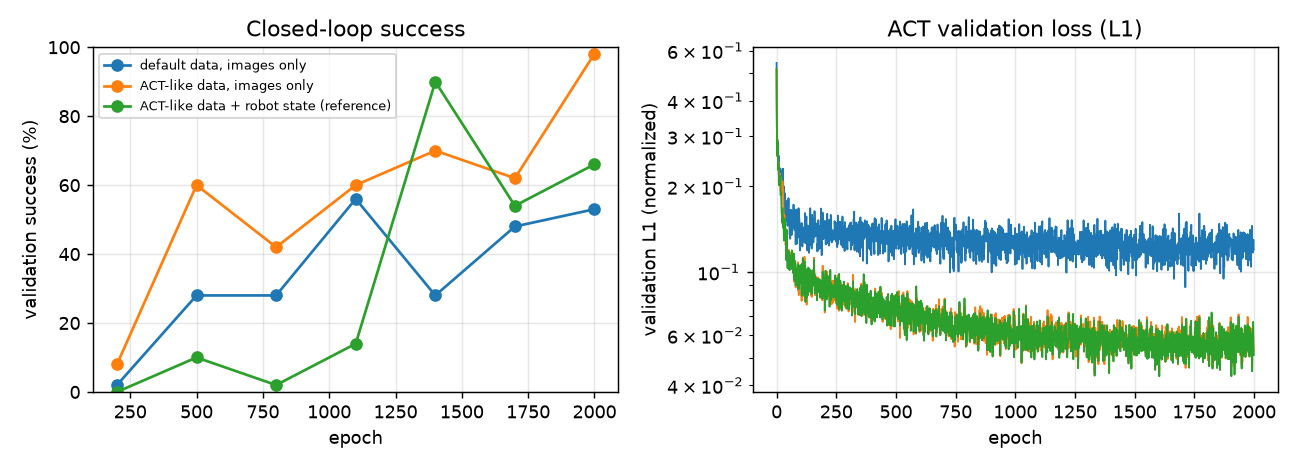
\includegraphics[width=\linewidth]{../experiments/act_original_curves.png}
  \caption{Validation success per epoch (50 rollouts; 100 at the last epoch) and ACT's
  validation loss for the three baseline runs. The loss is smooth while success varies
  between nearby checkpoints.}
  \label{fig:curves}
\end{figure}

\subsection{Execution ablation}
Table~\ref{tab:execution} compares four ways of executing the same policy's 20-action
chunks. Temporal ensembling is essential: executing each chunk open loop, as the
proposal planned, drops success from 98\% to 41\%, and re-querying more often without
averaging is worse.

\begin{table}[t]
  \caption{Execution of the 20-action chunks: deterministic-data policy, 100 source
  validation rollouts, one seed.}
  \label{tab:execution}
  \centering
  \small
  \begin{tabular}{@{}lr@{}}
    \toprule
    Execution & Success \\
    \midrule
    Temporal ensembling, $k = 0.01$ (used everywhere) & \textbf{98\%} \\
    Open loop: whole chunk, then re-query (proposal) & 41\% \\
    Re-query every 10 steps & 32\% \\
    Re-query every step, first action only & 1\% \\
    \bottomrule
  \end{tabular}
\end{table}

\subsection{Inverse dynamics model}
\todo{Table: IDM error per action component on held-out source transitions, and
pseudo-label error on each target, for $\lambda = 0$ (b) and DANN (c); three seeds.}

\subsection{Comparison with alternatives}
Table~\ref{tab:main} will hold the comparison on the C4 constraints (C9, C10).

\begin{table}[t]
  \caption{Test success (mean $\pm$ standard deviation over three seeds, 100 rollouts
  each), R4 gap closed and R5 retention drop. \todo{Fill; add targets B and C.}}
  \label{tab:main}
  \centering
  \small
  \begin{tabular}{@{}l@{\hspace{4pt}}lcccc@{}}
    \toprule
    & Method & Source & Target A & R4: $G_{\mathrm{A}}$ & R5: drop \\
    \midrule
    (a) & Source only & \todo{} & \todo{} & 0 (ref.) & 0 (ref.) \\
    (b) & Unadapted IDM & \todo{} & \todo{} & \todo{} & \todo{} \\
    (c) & DANN-adapted IDM & \todo{} & \todo{} & \todo{} & \todo{} \\
    (d) & Oracle & \todo{} & \todo{} & 1 (ref.) & \todo{} \\
    (e) & Augmentation & \todo{} & \todo{} & \todo{} & \todo{} \\
    \bottomrule
  \end{tabular}
\end{table}

\todo{Text: which methods meet R4 and R5 on each target; (b) against (c); (e) against
(c); latency for every method (R6); negative transfer if alignment hurts.}

\section{Discussion and Conclusions}
\label{sec:discussion}
% Interpret results, state whether the C4 constraints were met and why.
% C11: limitations and advantages.

\paragraph{Were the constraints met?}
So far R3 and R6 are met by the baseline, with a wide margin for R6, and R2's 80\% level
is met at 300 demonstrations. \todo{R1, R2 decision, R4 and R5 with the final results.}

\paragraph{Demonstration variability dominates.}
The same code and data budget give 99\% or 53\% depending on how the demonstrations
were generated. The ACT paper reports the same direction between scripted and human
demonstrations \citep{zhao2023act}. For this project it means that the quality of the
source data, not the policy architecture, decided whether the study was possible.

\paragraph{Validation loss does not select good policies.}
In every run, with both our reimplementation and the original ACT, the checkpoint with
the lowest validation loss succeeded less than the final one (for example 61\% against
98\%). The loss curve is smooth while success varies between nearby checkpoints.
Selection therefore needs closed-loop rollouts, which is cheap in simulation and costly
on a real robot. \todo{Cite prior reports of this effect (not yet in the bibliography).}

\paragraph{What went wrong.}
\label{sec:whatwentwrong}
We first wrote our own image-only ACT with the proposal's settings: joint increments,
chunks of 10 executed open loop, stochastic demonstrations. With 100, 200 and 300
demonstrations it reached 23\%, 49\% and 31\% validation success (one seed each); even
from training initial states it succeeded only 60--70\% of the time, and most failures
were missed grasps. Temporal ensembling made it worse (21\% and 14\% for 200 and 300
demonstrations), because averaging increments predicted from different states is not
well defined. Comparing against the original ACT pointed to the action representation,
the execution scheme and the demonstrations, not to training length. Running the
original code with absolute targets and deterministic demonstrations solved the source
task. The proposal's plan to execute chunks open loop would have cost 57 points.

\paragraph{Limitations.}
\begin{itemize}
  \item \textbf{Simplified task.} The object's yaw, the arm's start pose and the expert's
  speed are fixed, and the start area is $20 \times 20$~cm. The stochastic reference
  (53\%) shows that the baseline does not yet handle stock OCBench variability.
  \item \textbf{Simulation only.} Target videos come from the same simulator and expert
  as the source, so the only shift is the object. Real or generated videos add shifts
  in appearance and dynamics that we do not study.
  \item \textbf{Evaluation noise.} GPU rendering is not bit-exact: two renders of the
  same state can differ by one intensity level in a few pixels. With our earlier
  reimplementation this flipped 11 of 40 episode outcomes when the same seeds were
  rerun. We report intervals and never compare single reruns.
  \item \textbf{Seeds.} Current numbers use one training seed, and success varies between
  checkpoints of one run. \todo{Update after three seeds.}
  \item \textbf{Adversarial alignment.} DANN aligns marginal feature distributions; it
  does not guarantee that actions remain readable from the aligned features
  \citep{zhao2019invariant}, and it is weaker for regression than for classification
  \citep{nejjar2023daregram}. Per-component IDM errors test this. \todo{Outcome.}
  \item \textbf{Operations.} The original ACT code cannot resume, so a preempted cloud
  run restarts from zero.
\end{itemize}

\paragraph{Advantages.}
The design needs no target labels, no simulator state and no pretrained model; the IDM
runs offline, so the deployed policy costs the same as the baseline (10~ms per call).
Every comparison shares data, seeds, initial states, policy code and selection rule, and
the protocol was fixed before the results. Data, checkpoints and code are public.
\todo{Advantages supported by the final results.}

\paragraph{Conclusion.}
\todo{Answer the research question: do action-free videos, labeled by an adapted IDM,
close the gap to the oracle on each target while retaining the source?}

\section*{Contributions}
All members collaborated on and reviewed the report.
\todo{Update to what each member did.}

\begin{center}
\small
\begin{tabular}{@{}>{\raggedright\arraybackslash}p{2.6cm}>{\raggedright\arraybackslash}p{3.2cm}>{\raggedright\arraybackslash}p{6.7cm}@{}}
\toprule
Member & Role & Tasks \\
\midrule
Brik Meza & Data and evaluation & Simulation, expert demos, datasets, splits, rollouts, metrics \\
Myriam Dardour & Adversarial adaptation & Discriminator, adversarial training, tuning, experiments \\
Zheng Ye Zhang & Inverse dynamics model & IDM architecture and training, pseudo-labeling, error analysis \\
Gonzalo Mill\'an Garc\'ia & Baselines and alternatives & Policy training, baselines, alternative methods, comparisons \\
\bottomrule
\end{tabular}
\end{center}

\section*{Generative AI disclosure}
% Required by the course: disclose and justify any generative-AI use
% (McGill GPS guidelines). Must match docs/ai-use-log.md.
We used ChatGPT and Codex (OpenAI) and Claude and Claude Code (Anthropic), following
McGill's guidelines on generative AI in research. They assisted with (i) the literature
search and bibliography formatting; (ii) document structure and draft prose of the
proposal and this report; (iii) software: simulator changes in our OCBench fork, seeded
data collection and replay checks, dataset publishing, the training and evaluation
infrastructure, a first ACT reimplementation and its diagnostics, the adapter that runs
the original ACT, and tests; and (iv) running and summarizing the baseline experiments
that a team member approved. We used them to cover more engineering than a four-person
course project otherwise allows, so that the team's time went to design decisions and
analysis. The team directed the work, made the design decisions (scene, data sizes,
protocol, ACT settings) and approved every paid run. Verification: automated tests,
exact replay of stored episodes, end-to-end training and evaluation tests, and an
independent review of the ACT adapter against the upstream code; every reported number
comes from logged runs. The team revised the text and checked claims and citations
against the sources. \todo{Update from docs/ai-use-log.md before submission, including
the IDM and DANN work.}

\bibliographystyle{unsrtnat}
\bibliography{../references}

\end{document}
